% status: 100
% chapter: Twitter


\def\paperstatus{100} % a number from 0-100 indicating your status. 100
                % means completed
\def\paperchapter{Twitter} % This section is typically a single keyword. from
                   % a small list. Consult with theinstructors about
                   % yours. They typically fill it out once your first
                   % text has been reviewed.
\def\hid{hid-sp18-507} % all hids of the authors of this
                                % paper. The paper must only be in one
                                % authors directory and all other
                                % authors contribute to it in that
                                % directory. That authors hid must be
                                % listed first
\def\volume{9} % the volume of the proceedings in which this paper is to
           % be included

\def\locator{\hid, Volume: \volume, Chapter: \paperchapter, Status: \paperstatus. \newline}

\title{Analyzing Twitter Activity to Identify Spam Accounts}


\author{Stephen Giuliani}
\affiliation{%
  \institution{Indiana University}
  \state{Virginia}
  \country{USA}
}
\email{sgiulian@iu.edu}

\renewcommand{\shortauthors}{S. Giuliani}


\begin{abstract}
  This paper provides an analysis of Twitter account activity to
  identify potential spamming bots as opposed to organic user
  activity. The approach uses a combination of web scraping in python,
  data storage within the MongoDB Atlas Cloud, and implementing a REST
  service to pull data from the cloud, expose it on a local system,
  and then archive the data for analysis.
\end{abstract}

\keywords{\locator\ Twitter, MongoDB, REST, TweePy}


\maketitle

\section{Introduction}

The 2016 US Presidential election is a prime example of how social media can be
used to push an agenda or advertise specific points of view in such a volume
that discrediting the masses of inaccurate posts, shares, and re-tweets is a
near impossible feat. Many individuals, organizations, as well as government
entities, have utilized social media to flood various social mediums with
repetetive posts and comments at the hands of automated bots, rather than
real-user activity~\cite{WPostTwitterBots}. Since the unethical use of social
media in this manor has come to light, post election, the US Department of
State (DoS) and the Federal Bureau of Investigation (FBI) has been tasked to
identify and address the use of fake accounts to push political agendas and
manipulate the media as a whole~\cite{FBISocialMediaInvestigation}.

Luckily for investigators, account activity for automated or fake users is
typically characteristically different from the activity of organic or real
users~\cite{BDSTwitterBots}. This paper will provide an analysis on Twitter
users' accounts and user-habits to identify potential bots. This paper will
also identify certain topics that are more likely to fall victim to the
spamming tactics than less polar-opinion subject matter.

\section{Bots, Spam, and the Impact}

Automation is a norm in technology, especially social media. The purpose of the
automated account, or bot, is what determines whether the account is considered
spam versus a service. Examples of more favorable automated accounts include
the `Earthquake Bot', which automatically tweets warning information to areas
where a 5 or greater magnitude earthquake is detected, the `Netflix Bot', which
will notify you each morning of the latest Netflix releases, and the `Big Ben
Clock', which just tweets `BONG' every time London's Big Ben
chimes~\cite{cooltwitterbots}. The fun and useful bots are just a few examples
of how Twitter accounts can be used for a collectively positive purpose. In
contrast, there are accounts that serve only to like, re-tweet, or even produce
original content, at a higher daily rate and often focus on subject that are
hot-topics in the news or polarized views in politics. Within this analysis, we
have concluded that certain topics are more likely to have a spam bot presence
than others. For instance, `\#LockHerUp', a notorious hashtag used in favor of
putting Hillary Clinton in jail, is used by bots significantly more than
`\#SundayBrunch'.

The accounts that can be considered spam-based bots have similar account
behavior to other bots and can be classified collectively via just a few data
points. A spam bot is more likely to post at a much higher volume than a real
user. Some bots rack up high counts of re-tweets with very few original posts,
have a very unbalanced ratio of followers to people who follow back, and may
achieve a high volume of activity within a few days of creation.

The use of these spaming accounts creates artificial interest, or hype in
specific subjects. This tactic can keep topics in the limelight or falsely
overpower reputable news sources ultimately controlling what we see online or
in mainstream media~\cite{wikitwitterbot}. Instances where the masses latched
onto the volume of information rather without investigating source or
information independently can lead to dangerous conclusions and sometimes
unjustified courses of action. In 2012, the moments immediately following the
unfortunate incident at Sandy Hook lead to an online hunt and prosecution of
Ryan Lanza.  Varieties of social mediums were quick to post and share than Ryan
was the perpetrator of the terrorist attack, including death threats and
pledges of revenge. However, as a short time passed and sources were verified
and facts pushed through the social hype, Adam Lanza, Ryan's brother, was
identified as the shooter--well after news outlets followed and falsely
reported on socially-based conclusions~\cite{SandyHookForbes}.

\section{Analytical Approach}

In this section we will provide an overview of the primary steps involved in
acquiring, storing, querying, and analyzing the subject Twitter data.  

\textit{\bf Note to the reader:} 
In order to create, and therefore replicate, this paper, independent Twitter,
Gmail, and Twitter Developer accounts were created. These accounts and 
credentials are necessary for access to Twitter's API. Additionally, a 
temporary access account was set up so that instructors and reviewers could 
access and replicate data storage and pulls within the MongoDB Atlas cloud 
service. The credentials and access information is provided within the project
code and no changes should be made.

\subsection{Technologies Used}

\textit{\bf   Twitter API}

Twitter uses a publicly available API for all of its users' Twitter activity
and profile information. Free developer accounts are available and come with
the ability to pull data from the past 7 days. Increased scope is available
through paid-tiers of developer accounts.  \\ \textit{\bf Python: TweePy}

Tweepy is a package developed for the purpose of interacting with Twitter's
online API~\cite{PythonTweePy}. Queries are returned in JSON format for
analysis or direct storage.  \\ \textit{\bf MongoDB Atlas}

MongoDB is a popular NoSQL document database program that is open source and
can be deployed almost anywhere. MongoDB Atlas is a cloud-based MongoDB service
that can host documents through the services of Amazon Web Services (AWS),
Microsoft's Azure, or Google's Cloud Platform (GCP)~\cite{MongoDBAtlasPython}.
For purposes of this paper and analysis, we have used MongoDB Atlas to host the
scraped Twitter data, using AWS, and expose the data through a RESTful service.
\\ \textit{\bf Python: Flask (REST)}

Flask is a micro framework for Python that can be used to design and make
RESTful queries. We use flask to make GET requests to the MongoDB Atlas Cloud
data~\cite{MongoDBFlask}. The data requested is used for the analysis itself.
Once the data is scraped and stored within the cloud, python and Flask expose,
or makes available, the data on a predetermined web address, or local endpoint
for purposes of this paper.

\subsection{Web Scraping, Twitter Data}

In order to pull data from Twitter's API, you must first register for a
developer account (free). Once registered, and after creating a default
application, the account keys and credentials are necessary for authentication
when using tweepy in python. A free developer's account has the ability to pull
twitter data from the past 7 days only. For purposes of this analysis, these
seven days are sufficient. Documentation on the data Twitter makes available to
the public is available here~\cite{TwitterAPI}. Using tweepy, we are able to
query Twitter's data via a number of characteristics: hashtags, words present
in tweets, usernames, dates, and more. The JSON object that is returned
(dependent on the structure of the query) includes information on the user's
account since creation as well as meta-data on the tweet itself (geotags,
platform used to post, links used, and more). The entirety of the returned JSON
object is what is stored on the MongoDB Atlas cloud.

A typical Twitter query JSON object is less than 8 kB at a length of about 212
lines of code, based on a JSON dump of 100 tweet-data returns. Therefore, a
high volume of twitter data can be pulled in stored within the cloud for
analysis.  However, according to Twitter's API
policy~\cite{TwitterRateLimiting}, only 500 instances can be queried at once
with a registered development user (paid options available for higher volume
queries).

\subsection{MongoDB Atlas, Storing Twitter Data}

MongoDB's online web-hosting cloud service is available for free for testing
purposes. The limitations of this service is a 3-cluster database with a
storage limit of 512 Mb. Any requirements to use more than 3 clusters or
storage needs greater than 512 Mb requires paid subscriptions, which are
hourly-usage based.  The data scraped from Twitter will be stored on this cloud
and will be available to readers/reviewers after the analysis is concluded. For
purposes of demonstration and this paper, the query max of 500 instances will
be stored and used for the analysis. However, at an average of 8kb per tweet
query, over 64,000 instances can be stored within the free 512 Mb of data
MongoDB Atlas offers.

The ability to store data on a MongoDB database comes from the use of pymongo,
a Python package developed for the administration of Mongo
databases~\cite{PyMongoPython}. However, for testing purposes, we also used the
mongo-shell capabilities to clear, start, stop, and monitor the cloud-server
status. Documentation on pymongo and mongo-shell are available at
\url{https://api.mongodb.com/python/current/}.

Connection to the cloud database requires ssl authentication, which will be
published within this paper for testing purposes. Administration or viewing
permissions will also be created. The JSON objects produced within Python using
tweepy are stored in a created database collection on the Atlas cloud. This
cloud database is also use as the connection for the RESTful service to pull
specific data-points.

\subsection{Flask, RESTful Service in Pulling from the Cloud}

The data or JSON-format documents stored on the Atlas cloud can be connected to
and authenticated via pymongo in python. Flask is used to bridge the connection
and expose an available address for data to be displayed/used for
analysis~\cite{FlaskREST}. The RESTful API and paths created were created from
scratch, grouping specific JSON attributes of the stored data. For instance, in
order to determine the daily rate of posts per user, the GET request will pull
the data for the user's total posts and the data including the creation date of
the account. The JSON object produced via the GET request can be parsed and
regrouped prior to exposing the data on flask's default local endpoint. See the
code-documentation for the REST API used to query the Atlas cloud.

\subsection{Data Analysis}

As mentioned above, the data on the cloud can be pulled via GET requests. The
data required is pulled via specific GET requests so that analysis can be done.
MongoDB's Atlas cloud service has the ability to perform analysis on the cloud;
however a free testing account is not able to perform this. Therefore, the
analysis is conducted locally, via python objects. For purposes of data
familiarization, the data is pulled and stored in a comma-separated values
(CSV) format. This enables seamles interpretation by python's many analytical
and visual packages. Metrics such as daily rates for friending other users and
posting, friends-to-followers ratios, and account age are calculated. Medium, a
popular online publication and editorial provides ``Twelve Ways to Spot a
Bot''~\cite{HowToSpotABot} on Twitter; many of these points can be verified via
Twitter's public API data. For analytical purposes, the GET request, hosted by
flask through localhost endpoints, is downloaded as a raw JSON object and
converted and stored locally as a CSV. This paper will analyze the scraped
users' average posts per day, average favorites per day, as well as the ratio
of friends to followers. Spam bots are known to constantly produce tweets or
retweets and therefore we can expect a high number of average daily posts or
favorites per bot-users. Similarly, a spam bot often will follow, or friend, a
high volume of other twitter users so that its account expose increases. In
contrary to the number of friends a bot may have, the number of users that
follow back are usually low; therefore a high ratio of friends to followers can
indicate an automated account.

\section{Results}

Evaluating the average daily posts, average daily favorites, and ratio of
friends to followers revealed a majority of organic users; however there is
still a significant number of users identified as a possible spam bot. The
following tables, Table~\ref{t:post-summary}, Table~\ref{t:faves-summary}, and
Table~\ref{t:ratio-summary},  show the summary information on the daily post,
daily favorites, and friend to follower ratio data, respectively, pulled from
Twitter's user data. 

\begin{table}[htb]
\centering
\caption{Summary: Daily Posts}
\label{t:post-summary}
\begin{tabular}{lr}
Count & 460 \\
Mean  & 43.60  \\
Std   & 72.19  \\
Min   & 0.0014 \\
25\%  & 4.95   \\
50\%  & 17.49  \\
75\%  & 50.57  \\
Max   & 763.09
\end{tabular}
\end{table}

\begin{table}[htb]
\centering
\caption{Summary: Daily Favorites}
\label{t:faves-summary}
\begin{tabular}{lr}
Count & 460  \\
Mean  & 52.23  \\
Std   & 89.20  \\
Min   & 0.0024 \\
25\%  & 7.84   \\
50\%  & 23.02  \\
75\%  & 59.53  \\
Max   & 844.67
\end{tabular}
\end{table}

\begin{table}[htb]
\centering
\caption{Summary: Friends per Followers}
\label{t:ratio-summary}
\begin{tabular}{lr}
Count & 460 \\
Mean  & 1.53   \\
Std   & 1.77   \\
Min   & 0.00   \\
25\%  & 0.88   \\
50\%  & 1.09   \\
75\%  & 1.50   \\
Max   & 18.50 
\end{tabular}
\end{table}

Note that the number of instances within the CSV files totals only 460, rather
than the 500 available within the GET requests. This is because 40 posts are
associated with duplicate accounts that are already a part of the queried data;
therefore their data is duplicative and only requires a single instance for
evaluation. 

Users' post, favorites, and ratio data indicates right-skewed data points
because the minimum and maximum values are so far apart. The averages produced
are likely inaccurate for organic-only accounts. The standard deviation from
each of the means also indicates the wide range of account activity.

The histograms from Figures~\ref{f:post-hist},~\ref{f:faves-hist},
and~\ref{f:ratio-hist} support the summary data and the conclusion that some
accounts are not indicative of an average user.

\begin{figure}[!ht]
  %\TODO{THIS IMAGE IS MISSING}
  \centering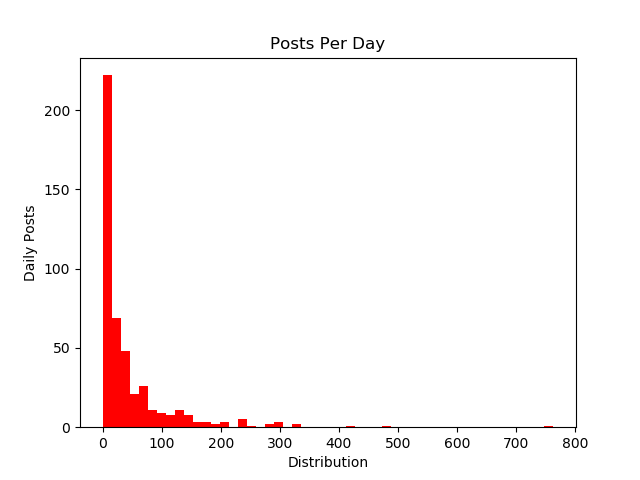
\includegraphics[width=\columnwidth]{images/post_hist.png}
  \caption{Histogram: Posts per Day}\label{f:post-hist}
\end{figure}

\begin{figure}[!ht]
  %\TODO{THIS IMAGE IS MISSING}
  \centering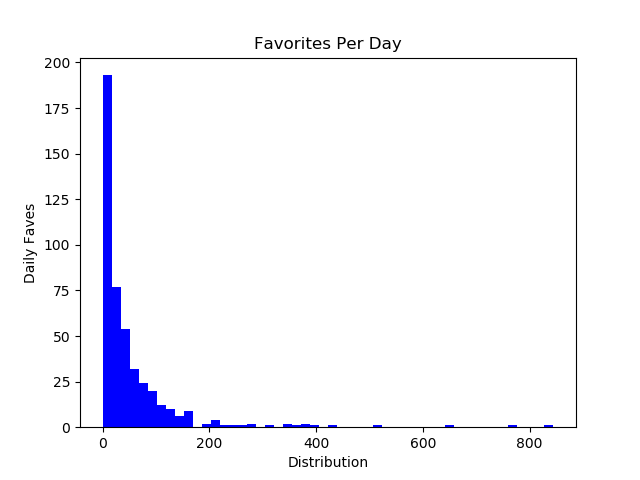
\includegraphics[width=\columnwidth]{images/faves_hist.png}
  \caption{Histogram: Favorites per Day}\label{f:faves-hist}
\end{figure}

\begin{figure}[!ht]
  %\TODO{THIS IMAGE IS MISSING}
  \centering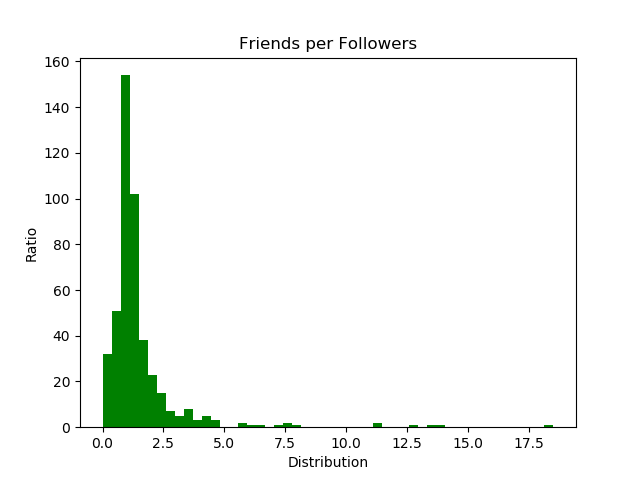
\includegraphics[width=\columnwidth]{images/ratio_hist.png}
  \caption{Histogram: Friends per Followers}\label{f:ratio-hist}
\end{figure}

Arbitrary metrics for differentiating activity of a spam-bot versus an organic
user we used to re-evaluate the data to filter out potential bots, or outliers,
in the queried data.

Daily posts of an organic user is considered to be at most 96 posts per day (a
user who posts a single tweet every 10 minutes for 16 hours each day).
Favorites per day was evaluated at a similar cap, only it was increased by 25
percent to account for the simplicity and efficiency of a favorite over a
produced tweet.  The ratio of friends to followers was capped at 2 times the
standard deviation of the original data, or about 3.5. This indicates that an
account may follow three and a half times as many users as are willing to
follow them. 

After filtering out the users that don't fall within these thresholds,
Table~\ref{t:post-delta}, Table~\ref{t:faves-delta}, and
Table~\ref{t:ratio-delta} show the delta, or change in the data as impacted by
the potential bot accounts.

\begin{table}[htb]
\centering
\caption{Adjusted: Daily Posts}
\label{t:post-delta}
\begin{tabular}{lr}
Count & 59  \\
Mean  & 21.59  \\
Std   & 48.79  \\
Min   & 0.00   \\
25\%  & 1.12   \\
50\%  & 4.32   \\
75\%  & 17.88  \\
Max   & 667.62
\end{tabular}
\end{table}

\begin{table}[htb]
\centering
\caption{Adjusted: Daily Favorites}
\label{t:faves-delta}
\begin{tabular}{lr}
Count & 47  \\
Mean  & 22.34  \\
Std   & 59.60  \\
Min   & 0.00   \\
25\%  & 1.55   \\
50\%  & 3.67   \\
75\%  & 13.18  \\
Max   & 726.27
\end{tabular}
\end{table}

\begin{table}[htb]
\centering
\caption{Adjusted: Friends per Followers}
\label{t:ratio-delta}
\begin{tabular}{lr}
Count & 28 \\
Mean  & 0.35  \\
Std   & 1.14  \\
Min   & 0.00  \\
25\%  & 0.04  \\
50\%  & 0.03  \\
75\%  & 0.09  \\
Max   & 14.98 
\end{tabular}
\end{table}

As shown in Table~\ref{t:post-top10}, Table~\ref{t:faves-top10}, and
Table~\ref{t:ratio-top10}, the average for daily posts and daily favorites fell
by more than half the original mean. Of the 59, 47, and 28 accounts that were
filtered out per each category, the top ten and the values that flagged them
are shown below.

\begin{table}[htb]
\centering
\caption{Potential Bots: Criteria = Daily Posts}
\label{t:post-top10}
\begin{tabular}{lr}
Screen Name & Avg. Daily Posts \\
\toprule
MaheshC78848209 & 763.09  \\
KatTheHammer1   & 475.44  \\
GaryWil29548846 & 421.00  \\
DonGibs22787443 & 330.10  \\
ARealPrincesa   & 327.32  \\
notbuyingthat54 & 304.66  \\
nice-centurion  & 294.95  \\
lynn85706529    & 291.30  \\
FrankJManrique3 & 287.52  \\
R98250729       & 279.81  
\end{tabular}
\end{table}

\begin{table}[htb]
\centering
\caption{Potential Bots: Criteria = Daily Favorites}
\label{t:faves-top10}
\begin{tabular}{lr}
Screen Name & Avg. Daily Favorites \\
\toprule
siminuteman1776 & 844.67 \\
ImmoralReport   & 772.75 \\
MaheshC78848209 & 644.52 \\
KatTheHammer1   & 522.71 \\
GaryWil29548846 & 427.00 \\
4Freedom4ever   & 395.86 \\
mickeyh54099794 & 380.63 \\
FrankJManrique3 & 374.21 \\
lynn85706529    & 368.90 \\
melinda63312935 & 350.65  
\end{tabular}
\end{table}

\begin{table}[htb]
\centering
\caption{Potential Bots: Criteria = Friends per Followers}
\label{t:ratio-top10}
\begin{tabular}{lr}
Screen Name & Friends per Followers \\
\toprule
Andy75213017    & 18.50 \\
KenSR-802VT     & 13.75 \\
wesleyh23420956 & 13.44 \\
JamesChhetri7   & 12.58 \\
john316stv      & 11.46 \\
Ikram-35        & 11.25 \\
JaredFu88957380 & 7.87 \\
LDuvall19       & 7.59 \\
nateweyand      & 7.48 \\
DJLPX           & 7.31  
\end{tabular}
\end{table}

The analysis in each category was conducted independently. However, merging the
Top 10 candidate bots based on daily activity shows 5 accounts sharing the top
ten in both categories. When comparing the top 10 based on friend-follower
ratios, none of these users share the top 10 with the daily-activity-based top
10 accounts.

\section{Challenges and Opportunities}

The purposes of this paper are to demonstrate the ability to scrape, store,
access, and analyze data; however the analysis itself is only part of a much
larger potential research topic; one that is outside the scope of this course. 

\subsection{Challenges}

This paper demonstrates the ability to scrape and store data on the cloud where
the data can be pulled, exposed locally, and then downloaded into
analytical-friendly formats. Limitations on this analysis include Twitter's
policy for query frequency and size of the data returned as well as MongoDB
Atlas's limit on data storage. Both of these can be mitigated via paid
respective accounts. Additionally, in order to perform the analysis independent
of the provided credentials, a user must register themselves for these
services.  Also, depending on the query or subject matter of the requested
information, the freely available 7-day history might not suffice. Sentiment
analysis and bot filtering on past events would require the ability to pull
tweets or archived user data. 

\subsection{Opportunities}

In order to truly conclude a spam-bot over atypical organic user further
analysis should be conducted. Analysis can include re-querying Twitter for
specific users (such as the 5 that shared the top tens for daily activity)
where the data on a specific-user's tweets can be evaluated with sentiment
analysis, analysis on the repetition of tweets, other subjects the user
promotes, and the platforms and languages used to tweet. Bots typically are
based on programs that are not run using a mobile platform, such as the Twitter
app on a phone; contrarily, most organic twitter users use their phone as the
primary posting/sharing/favoring platform. Deep learning, out of scope of this
paper is a great opportunity to parse through the dense JSON object pulled per
user.

Additionally, some cloud services and platforms come with analytical
capabilities in house. The lowest tier within the MongoDB Atlas cloud service
does not offer data analytics; however should a cloud database platform be used
with these capabilities it would eliminate the need to re-pull data to a local
machine or server as the analytics, or even the necessary python files can be
hosted and executed directly from the cloud.

\section{Conclusion}

Clearly, automation within Twitter is prevalent. According to a study conducted
by the University of Southern California and Indiana University, up to 15\% of
twitter accounts could be bots~\cite{USCIUBotStudy}. Lately, the news, as well
as the FBI, have focused on the use of these bots as a way of manipulating
media and public perception. By pulling data from just the past seven days from
Twitter, based on a query for a hot-topic hashtag, `\#LockHerUp', and
determined by activity that deviates from typical organic user activity, over
100 accounts appear to be automated and in support of the politically-charged
campaign.

The ability to scrape, and directly store-then-pull data on MongoDB's Atlas
cloud service was seamless, efficient, and was possible at no cost to the user.
The 500 records pulled from Twitter and stored in the cloud occupied less than
1\% of the available memory cap and therefore allows for opportunities to
vastly increase data volumes for analysis. 

\begin{acks}

  The authors would like to thank Dr.~Gregor~von~Laszewski and the Associate
Instructors for their support and suggestions while writing this paper.

\end{acks}

\bibliographystyle{ACM-Reference-Format}
\bibliography{report} 
